% SPDX-License-Identifier: CC-BY-4.0
\documentclass[11pt,reqno]{amsart}

\usepackage[T1]{fontenc}
\usepackage{lmodern}
\usepackage[margin=1in]{geometry}
\usepackage{amsmath,amssymb,amsthm,mathtools}
\usepackage{booktabs,array,tabularx}
\usepackage{microtype}
\usepackage{xcolor}
\PassOptionsToPackage{obeyspaces}{url}
\usepackage{url}
% Break code/paths/URLs only at punctuation (never mid-word); long hex hashes use \hashcode.
\def\UrlBreaks{\do\.\do\/\do\-\do\_\do\:\do\=\do\,\do\{\do\}}
\def\UrlBigBreaks{}
\Urlmuskip=0mu plus 1.0mu
\usepackage{tikz}
\usetikzlibrary{arrows.meta,positioning}
\usepackage[colorlinks=true,linkcolor=blue!60!black,citecolor=teal!60!black,urlcolor=blue!60!black,pdftitle={The Unsolved Mathematics Atlas (v0.10.0): Six-Kernel Formal Core, Asymmetric Hydra, and Audit},pdfauthor={Alexander S. Donahue}]{hyperref}

\emergencystretch=3em
\tolerance=1500
\raggedbottom

\theoremstyle{plain}
\newtheorem{theorem}{Theorem}[section]
\newtheorem{lemma}[theorem]{Lemma}
\newtheorem{proposition}[theorem]{Proposition}
\newtheorem{corollary}[theorem]{Corollary}
\theoremstyle{definition}
\newtheorem{definition}[theorem]{Definition}
\newtheorem{remark}[theorem]{Remark}

\newcommand{\Z}{\mathbb{Z}}
\newcommand{\N}{\mathbb{N}}
\newcommand{\Q}{\mathbb{Q}}
\newcommand{\R}{\mathbb{R}}
\newcommand{\code}[1]{{\upshape\nolinkurl{#1}}}
\newcommand{\hashcode}[1]{{\upshape\def\UrlBreaks{\do\:\do 0\do 1\do 2\do 3\do 4\do 5\do 6\do 7\do 8\do 9\do a\do b\do c\do d\do e\do f\do h\do n\do p\do s\do w}\nolinkurl{#1}}}

\title[The Unsolved Mathematics Atlas (Version 0.10.0): Six-Kernel Formal Core \& Hydra]{%
  The Unsolved Mathematics Atlas (Version 0.10.0):\\
  A Standalone Eight-Domain, Six-Kernel\\
  Lean 4.35.0 Formal Core, Catalytic \& Asymmetric Hydra Collatz Suite,\\
  Citation Audit, and Epistemic Verification Framework}

\author{Alexander S. Donahue}
\address{Independent Researcher, Spokane, WA, USA}
\email{0\_0@0thernes.art}
\urladdr{https://github.com/0thernes/unsolved-mathematics}
\thanks{ORCID: \href{https://orcid.org/0009-0006-8168-9648}{\texttt{0009-0006-8168-9648}}.
Repository release \texttt{v0.10.0} (November 27, 2026; Archive ID \texttt{0TH-BUILD-004};
Lean 4.35.0 commit \hashcode{eb6cafb7290e8bd5f2937522d8d804f58f02bafc}; Software Heritage prior
snapshot \hashcode{swh:1:snp:c11ec8263dd64b986c52bb400b8c3a85a3e6a254}).
All Lean 4.35.0 proofs, C17/Rust kernels, and Python tools are MIT-licensed; original prose, tables,
and datasets are CC BY 4.0 (with the third-party \code{data/external/lefttosolve/} mirror carved
out per \code{LICENSE}). Transparent AI-assistance, export-control, and conflict-of-interest
disclosures appear in Section~\ref{sec:governance}.}

\subjclass[2020]{Primary 03B35, 11B83, 11A25, 11D68, 11D61; Secondary 05D10, 11A41, 11J71, 68V15, 68V20}
\keywords{Lean 4, multi-kernel verification, Collatz conjecture, Fine--Wilf theorem, catalytic
computing, Euclid--Euler theorem, Mersenne prime divisors, Erd\H{o}s--Straus conjecture, Lonely
Runner conjecture, Brocard's problem, Ramsey theory, citation verification, RFC 3161 timestamps,
FAIR datasets, epistemic hygiene}

\begin{document}

\begin{abstract}
Large language models can rapidly draft mathematical surveys, yet unverified AI-assisted
corpora suffer systematically from fabricated bibliographic identifiers, unhedged proof claims,
definitional drift, silent indexing collisions, and opaque provenance. We present
\textbf{The Unsolved Mathematics Atlas} (\texttt{v0.10.0}), an open, reproducible, FAIR-indexed
catalog of 120 unsolved mathematical problems across 38 fields paired with an end-to-end
epistemic verification stack. Our contributions are fourfold.
First, live primary-source auditing across 646 identifier-bearing rows verified \textbf{537}
identifiers via arXiv and Crossref APIs in exact 1-to-1 bijection with all 120 \code{papers.md}
tables (445 in the initial 554-row sweep, 86/86 in 14 new \texttt{v0.8.0} dossiers, and 11/11
live-verified replacements/bijection closures in \texttt{v0.8.2}, zero duplicate or bare IDs)
while purging \textbf{109 invalid identifiers (19.7\% initial corruption, peaking at 36.4\% in
Dynamical Systems)}; Crossref/DataCite auditing of all \textbf{287} verified DOIs confirmed
\textbf{0 retractions} and logged \textbf{3 publisher errata}.
Second, we build a standalone, zero-Mathlib \textbf{Lean 4.35.0} formal core (\code{lean/},
\code{autoImplicit = false}) certifying \textbf{74 headline theorems}, 20 non-vacuity witnesses,
and 24 adversarial false-variant refutations (\textbf{118 audited declarations}, 16 zero-axiom)
across eight domains: Collatz (36 theorems, including chiral sign conjugacy
$T^d(-x) = -T_-^d(x)$, exact mod-3 chiral asymmetry, universal 3-adic intercept units, global
$3 \nmid x$ nonzero cycle exclusion, positivity localization, subcriticality, unconditional 1-,
2-, 3-, and 4-odd-step positive-cycle exclusion for all $d \ge 1$, sharp affine intercept and
Eliahou--Steiner cycle amplitude ceilings, $d \le 7$ exclusion, a Fine--Wilf 2-adic ceiling, and
catalytic cylinder evaluation), Erd\H{o}s--Straus (Mordell's 834/840 classes), Lonely Runner
(sharpness for all $n$ and the classical constructive proof for $n \le 3$), Brocard ($n \le 20$),
Primes/Twins, Goldbach ($n \le 100$), Perfect/Mersenne (complete Euclid--Euler with proved
$\mathrm{divSum}=\sigma$ and Euler's $2p \mid q-1$), and Ramsey ($R(3,3)=6$, $R(3,4)=9$). Proof
modules use zero \code{sorry}/\code{native_decide} (\code{Challenge.lean} holds the 74 \code{sorry}
specs), depend only on \texttt{\{propext, Classical.choice, Quot.sound\}}, and pass six Lean
kernels plus \code{lake comparator}. Third, we introduce a zero-workspace \textbf{C17/BMI2 + safe
Rust} Collatz accelerator and \textbf{Five-Vector Asymmetric Hydra} lab (fuzzed across 500,000
combined ASan/UBSan cases, 0 traps, 100\% bit-exact C17/Rust/Python parity), achieving
\textbf{1,683$\times$--7,137$\times$} wall-clock speedups ($t \le 26$: \textbf{884.4M} pairs in
$0.133$\,s; $d = 34$: \textbf{174.4M} DFS leaves in \textbf{4,096\,B} of stack), uncovering an
exact \textbf{Tropical Modular Mirror Law} ($\mu^*(2^a 3^b) = (a+b-1)/(a+b) \to 1$ vs.\
Archimedean box break $1/2 < \log_3 2 < 2/3$), a $+3.000$-bit carry-avalanche asymmetry, and the
$B \le 22$ Minimax Demon frontier ($0\%$ escape vs.\ $67.23\%$ for $3n-1$).
Fourth, Cross-Atlas auditing against \code{unsolved-problems-mega-atlas} (\texttt{v2.10.0},
2,000 problems) affirms \textbf{0/2,000} retirements across 56 archive entries, a daily sharded
mirror of all 26 Left to Solve programs (62,790 items) quarantines 4 unverified third-party
agent-claim review signals, and multi-cycle ten-class hardening achieves 104 passing tests,
10/10 mutation kill, 20/20 zero-error \code{mypy}, FAIR RO-Crate/Croissant metadata, and dual
RFC~3161 + Bitcoin OTS proofs over a 52-file SHA-256 manifest.
\textbf{No open conjecture in the catalog is claimed to be solved by this work.}
\end{abstract}

\maketitle

\section{Introduction, Epistemic Scope, and Claims Ledger}\label{sec:intro}

The proliferation of AI-assisted mathematical writing introduces an acute verification
asymmetry: generating a fluent survey or plausible proof sketch requires seconds, whereas
exposing a hallucinated DOI, an unstated Lean axiom, a hidden implicit variable, a vacuous
hypothesis, or a sign-blind Collatz heuristic requires disciplined mechanical infrastructure.
\emph{The Unsolved Mathematics Atlas} (\url{https://github.com/0thernes/unsolved-mathematics},
release \texttt{v0.10.0}) treats epistemic honesty and machine-checked falsifiability as its
primary engineering invariants.

To eliminate any ambiguity for human referees, institutional evaluators, or automated indexing
pipelines, we place our hard non-claim boundary at the front of this report:
\begin{quote}
\textbf{Explicit Non-Claim.} This paper and its companion repository solve \emph{zero} open
mathematical conjectures. Every formally verified theorem in \code{lean/} proves an exact
structural identity, classical foundation, modular reduction, sharpness bound, finite
exhaustion, or $3n-1$ sibling comparison (not a formal barrier theorem). Collatz (general
subcritical positive cycles with $o \ge 5, d \ge 9$ and divergent orbits), Erd\H{o}s--Straus
(general primes in Mordell's six square classes mod 840), Lonely Runner in general (proved for
up to 13 runners in recent preprints \cite{rosenfeld2025lonely8,trakulthongchai2025lonely910,
sungkawichai2026lonely1113}; the $n \le 3$ cases formalized here are classical
\cite{betkewills1972,cusick1973}), Brocard finiteness, Twin Primes, Goldbach's strong conjecture,
Odd Perfect Numbers, Mersenne Infinitude, and higher Ramsey numbers ($R(5,5)$ and diagonal
asymptotics) all remain \textbf{open}.
\end{quote}

Every substantive assertion in the repository is indexed in \code{CLAIMS.md} under six
epistemic tags (\code{kernel-checked}, \code{machine-checked-ci}, \code{primary-source-verified},
\code{computational-certificate}, \code{editorial-synthesis}, and \code{open-conjecture}), each
paired with an explicit falsification trigger. Table~\ref{tab:claims} reproduces the 1-to-1
numbered Claims Ledger (\code{C-01}--\code{C-14}) matching \code{CLAIMS.md}; post-release errors
and scope tightenings are logged append-only in \code{ERRATA.md} under a non-silent correction
and withdrawal policy.

\begin{table}[htbp]
\centering
\caption{Numbered Claims Ledger (1-to-1 Parity with \code{CLAIMS.md}, Release \texttt{v0.10.0}).}
\label{tab:claims}
\scriptsize
\setlength{\tabcolsep}{3.5pt}
\begin{tabularx}{\textwidth}{@{}l>{\raggedright\arraybackslash}p{3.4cm}>{\raggedright\arraybackslash}X>{\raggedright\arraybackslash}X@{}}
\toprule
ID & Epistemic Tag & Headline Claim & Falsification Trigger \\
\midrule
\code{C-01} & \code{machine-checked-ci} & Zero open conjectures claimed solved across active prose (120 dossiers) & Unhedged victory claim or missed fixture in \code{proof_claim_sweep.py} \\
\code{C-02} & \code{kernel-checked} & 74 theorems, 20 witnesses, 24 refutations (118 decls, 8 domains, \code{autoImplicit=false}) valid in 6 Lean 4.35.0 kernels + 3/3 neg rejection & Any kernel/comparator rejection, non-standard axiom, or failed negative probe \\
\code{C-03} & \code{kernel-checked} & Collatz 36-thm core: sign conjugacy, mod-3 chiral asymmetry, $3 \nmid c(w)$ \& $3 \nmid x$, 1-/2-/3-/4-odd \& $d\le 7$ exclusion, intercept/amplitude \& Fine--Wilf ceilings, catalytic eval & Supercritical $c(w)<3^o-2^d$, $3\mid x$ cycle, $o\le 4$/$d\le 7$ cycle $\notin\{1,2\}$, or ceiling violation \\
\code{C-04} & \code{kernel-checked} & Erd\H{o}s--Straus Mordell 834/840, closure, symmetry, $2\le n\le 30$, 6 squares & Counterexample outside 6 classes or cleared-denominator mismatch \\
\code{C-05} & \code{kernel-checked} & Lonely Runner $n\le 3$ + sharpness; Brocard $\le 20$; Primes/Twins; Goldbach $\le 100$; Complete Euclid--Euler \& $2p\mid(q-1)$; Ramsey $R(3,3)=6, R(3,4)=9$ & Arithmetic counterexample over $\Z/\Q$ or kernel rejection \\
\code{C-06} & \code{computational-certificate} & Catalytic C17/BMI2 + 5-Vector Asymmetric Hydra + safe Rust oracles ($t\le 26$, $d\le 34$, $B\le 22$, ASan/UBSan + 500k fuzz cases) are bounded diagnostics only & Parity mismatch, sanitizer/fuzzer trap, or failure in \code{test_collatz_instruments.py} \\
\code{C-07} & \code{primary-source-verified} & 537 identifiers API-verified in 1-to-1 log bijection (646 audited); 109 bad IDs purged; 0/287 DOIs retracted (3 errata) & Re-query returning 404, mismatch, duplicate, or retraction on a \code{verified} row \\
\code{C-08} & \code{primary-source-verified} & Statuses updated through 2026-11-27; 0/2,000 Mega-Atlas problems retired across 56 archive entries & Withdrawal of \code{2605.20695} or peer-reviewed settlement of an open entry \\
\code{C-09} & \code{editorial-synthesis} & CSS rankings are deterministic editorial heuristics, not objective depth scores & Non-deterministic ordering or cross-file CSS/rank drift \\
\code{C-10} & \code{machine-checked-ci} & 1/4 AI passes (Claude 2026-06-14, \code{claude-opus-4-8}) on initial 106; 14 \texttt{v0.8.0} pending; 0/120 human peer reviews & Any unlogged claim of independent multi-model or human peer sign-off \\
\code{C-11} & \code{machine-checked-ci} & Derived views \& 3,985 RAG chunks (822,897 tokens) deterministic, LF-only, zero local paths & Non-empty \code{git diff} after rebuild, duplicate chunk ID, or local path leak \\
\code{C-12} & \code{machine-checked-ci} & 104 passing tests (unit, neg, Hypothesis, oracle, metamorphic, external, native) + 10/10 mutation kill & Any failing regression test or surviving mutant in \code{mutation_check.py} \\
\code{C-13} & \code{machine-checked-ci} & 52-file SHA-256 manifest, DigiCert \code{.tsr} + Bitcoin \code{.ots}, SWHID, and SLSA release & Hash/imprint mismatch or invalid SLSA provenance attestation \\
\code{C-14} & \code{machine-checked-ci} & Daily full 26-program / 62,790-item mirror (27 $<4$\,MB shards, 4 agent-claim signals quarantined) never alters Atlas status & \code{--check} failure, shard $\ge 5$\,MB, excerpt leak, or mirror-driven status change \\
\bottomrule
\end{tabularx}
\end{table}

\section{Atlas Registry, Deterministic Scoring, and FAIR Architecture}\label{sec:atlas}

The sole canonical source of truth is \code{data/problems.yaml}, cataloging 120 open
mathematical problems across 38 fields (expanding from 106 in \texttt{v0.7.0} by adding 14
flagship open problems drawn from \code{google-deepmind/formal-conjectures} / Left to Solve:
four Erd\H{o}s Prize problems, nine Wikipedia formal targets, and the OEIS Riesel problem),
validated strictly against \code{schema/problem.schema.json} (JSON Schema Draft 2020-12). All
derived artifacts---\code{data/problems.json}, \code{RANKING.md}, the master table in
\code{README.md}, all 120 per-problem dossier headers, five cross-cutting indexes under
\code{docs/indexes/}, the interactive web explorer, Proof Blueprint, and programs mirror
(\code{_site/{index,blueprint,collatz-hydra,programs}.html}), and the offline BM25 retrieval corpus
(\code{rag/corpus.jsonl}, 3,985 unique chunks across 822,897 deterministic tokens)---are
generated reproducibly with zero-drift checks enforced on every CI push.

\subsection{Composite Severity Score (Editorial Heuristic)}
For navigational prioritization only---explicitly \emph{not} an objective measurement of
mathematical depth---each problem $p$ receives a deterministic Composite Severity Score
(rounded to three decimal places in \code{scripts/generate.py}):
\begin{equation}\label{eq:css}
  \mathrm{CSS}(p) = 0.40\,D(p) + 0.30\,C(p)
    + 0.20\,\min\!\Bigl(100,\;\max\!\Bigl(0,\,\frac{2026 - y_p}{3}\Bigr)\Bigr)
    + 0.10\,(100 - T(p)),
\end{equation}
where $D, C, T \in [0,100]$ are curated difficulty, centrality, and tractability ratings,
$y_p$ is the year posed (negative for BCE), and the reference year is frozen at $2026$ for
bit-for-bit reproducibility across calendar years. Ties break deterministically by lexicographic
slug order \code{(-css, slug)}. Table~\ref{tab:top15} lists the top 15 entries generated
verbatim from \code{data/problems.json}.

\begin{table}[htbp]
\centering
\caption{Top 15 Ranked Problems in \code{data/problems.json} (\texttt{v0.10.0}, 120 Problems, Frozen Reference Year 2026).}
\label{tab:top15}
\footnotesize
\setlength{\tabcolsep}{4pt}
\begin{tabular}{@{}rllrrl@{}}
\toprule
\# & Problem & Primary Field & Posed & CSS & Status \\
\midrule
 1 & The Riemann Hypothesis & Analytic Number Theory & 1859 & 89.933 & \code{open} \\
 2 & Goldbach's Conjecture & Number Theory & 1742 & 87.933 & \code{open} \\
 3 & The Grand Riemann Hypothesis & Analytic Number Theory & 1884 & 84.967 & \code{open} \\
 4 & Gauss Class Number (Real Quadratic) & Number Theory & 1801 & 83.400 & \code{open} \\
 5 & P versus NP & Computational Complexity & 1971 & 81.967 & \code{open} \\
 6 & The Hodge Conjecture & Algebraic Geometry & 1950 & 79.967 & \code{open} \\
 7 & The Twin Prime Conjecture & Number Theory & 1849 & 79.600 & \code{active-progress} \\
 8 & Birch and Swinnerton-Dyer Conjecture & Number Theory & 1965 & 78.867 & \code{open} \\
 9 & Existence of Odd Perfect Numbers & Number Theory & $-300$ & 78.300 & \code{open} \\
10 & The Dirichlet Divisor Problem & Analytic Number Theory & 1849 & 77.400 & \code{active-progress} \\
11 & Infinitude of Mersenne Primes & Number Theory & 1644 & 76.600 & \code{open} \\
12 & The Continuum Hypothesis & Set Theory \& Logic & 1878 & 76.267 & \code{independent} \\
13 & Hilbert's Sixteenth Problem (Part II) & Dynamical Systems & 1900 & 76.100 & \code{open} \\
14 & Yang--Mills Existence and Mass Gap & Mathematical Physics & 2000 & 75.333 & \code{open} \\
15 & Resolution of Singularities (Char.\ $p>0$) & Algebraic Geometry & 1964 & 75.033 & \code{active-progress} \\
\bottomrule
\end{tabular}
\end{table}

\subsection{Retrieval Hygiene, FAIR Metadata, and Dual Cryptographic Timestamps}
Forensic auditing of pre-\texttt{v0.3.0} releases exposed a silent key-collision defect in
\code{rag/build_corpus.py}: resetting chunk counters per Markdown heading produced duplicate
chunk IDs across roughly 80\% of multi-heading sections, silently overwriting vectors during
dense indexing. Replacing that logic with a monotonic per-\code{(slug, section)} counter
eliminated all duplicates (enforced by \code{scripts/validate.py} and regression-tested in
\code{tests/}). Release \texttt{v0.10.0} ships machine-readable FAIR dataset descriptors
conforming to \textbf{RO-Crate 1.1} (\code{ro-crate-metadata.json}) and \textbf{MLCommons
Croissant 1.0} (\code{croissant.json})---now checked directly by \code{validate.py} for version
parity against \code{VERSION}---plus dual third-party cryptographic timestamp proofs over
\code{data/MANIFEST.sha256}: a DigiCert RFC~3161 Time-Stamp Authority reply
(\code{data/MANIFEST.sha256.tsr}) and a 3-calendar Bitcoin OpenTimestamps proof
(\code{data/MANIFEST.sha256.ots}), both verified offline on every CI push and release tag via
\code{scripts/timestamp_manifest.py --check}.

\section{Empirical Primary-Source Citation and Retraction Audit}\label{sec:citations}

Because LLM-assisted literature compilation routinely hallucinates plausible yet nonexistent or
misattributed DOIs and arXiv IDs, \code{scripts/verify_citations.py} resolves every
identifier-bearing row across all 120 \code{problems/*/papers.md} tables live against
\code{export.arxiv.org} and \code{api.crossref.org}, verifying author and title overlap plus
publication year. To eliminate a secondary \emph{retraction blindspot}---wherein a valid DOI
has subsequently been retracted---\code{scripts/check_retractions.py} audits every verified DOI
against Crossref (\code{updated-by}, \code{update-to}, \code{relation}, and title notices) and
DataCite (\code{10.48550/*} arXiv DOIs).

\begin{table}[htbp]
\centering
\caption{Aggregate live primary-source citation audit and Crossref/DataCite retraction audit (\texttt{v0.10.0}).}
\label{tab:citations}
\footnotesize
\begin{tabular}{@{}lrr@{}}
\toprule
Audit Metric & Count & Share / Note \\
\midrule
Initial 106-dossier audit rows queried live & 554 & 100.0\% (0 network errors) \\
\quad API-verified (initial 106 dossiers) & 445 & 80.3\% (tagged \code{verified}) \\
\quad Author/title mismatch (purged \& downgraded) & 86 & 15.5\% (stripped to ``---'') \\
\quad Identifier not found / HTTP 404 (purged) & 23 & 4.2\% (stripped to ``---'') \\
\quad Invalid/hallucinated IDs eliminated (initial) & \textbf{109} & \textbf{19.7\% initial corruption} \\
New \texttt{v0.8.0} 14-dossier rows verified live & \textbf{86} & \textbf{100.0\% verified (0 bad)} \\
\texttt{v0.8.2} bijection closure (Collatz/bare/dup) & \textbf{+6 net} & \textbf{11/11 live; 4 dupes fixed} \\
Cumulative verified / total audited records & \textbf{537 / 646} & Exact 1-to-1 log bijection \\
\midrule
Verified DOIs audited for retraction notices & \textbf{287} & 100.0\% (0 network errors) \\
\quad Confirmed retractions / withdrawals & \textbf{0} & 0.0\% \\
\quad Publisher errata / corrections logged & 3 & Transparently recorded \\
\bottomrule
\end{tabular}

\smallskip
{\footnotesize Sources: \code{data/citation-verification-log.json} and \code{data/retraction-audit.json}.}
\end{table}

\subsection{Disaggregated Identifier Corruption by Mathematical Field}
Disaggregating the 554 live-audited rows by primary mathematical field (Table~\ref{tab:field_corrupt}
and Figure~\ref{fig:corrupt_chart}) reveals sharp structural heterogeneity: older journal-heavy
fields such as Dynamical Systems ($36.4\%$), Geometric Topology ($30.6\%$), and Mathematical
Physics ($30.0\%$) suffered roughly an order of magnitude higher LLM DOI hallucination rates
than arXiv-native fields such as Computational Complexity ($3.6\%$) and Probability Theory
($3.8\%$), while the human-and-tool-audited Collatz dossier recorded $0.0\%$ corruption ($0/15$).

\begin{table}[htbp]
\centering
\caption{Empirical Identifier Corruption Rates Across the 15 Highest-Volume Fields in
\code{data/citation-verification-log.json} (live arXiv + Crossref API resolution).}
\label{tab:field_corrupt}
\footnotesize
\begin{tabular}{@{}lrrrrr@{}}
\toprule
Primary Field & Checked & Verified & Mismatch & 404 & Corruption Rate \\
\midrule
Dynamical Systems & 22 & 14 & 6 & 2 & 36.4\% \\
Geometric Topology & 36 & 25 & 10 & 1 & 30.6\% \\
Mathematical Physics & 20 & 14 & 6 & 0 & 30.0\% \\
Combinatorial Geometry & 14 & 10 & 4 & 0 & 28.6\% \\
Harmonic Analysis & 27 & 20 & 6 & 1 & 25.9\% \\
Graph Theory & 28 & 21 & 6 & 1 & 25.0\% \\
Combinatorics & 20 & 15 & 1 & 4 & 25.0\% \\
Algebraic Topology & 16 & 12 & 2 & 2 & 25.0\% \\
Number Theory & 115 & 91 & 18 & 6 & 20.9\% \\
Knot Theory & 21 & 17 & 4 & 0 & 19.0\% \\
Partial Differential Equations & 16 & 13 & 2 & 1 & 18.8\% \\
Analytic Number Theory & 49 & 45 & 2 & 2 & 8.2\% \\
Probability Theory & 26 & 25 & 0 & 1 & 3.8\% \\
Computational Complexity Theory & 28 & 27 & 1 & 0 & 3.6\% \\
Number Theory / Dynamical Systems (Collatz) & 15 & 15 & 0 & 0 & 0.0\% \\
\bottomrule
\end{tabular}
\end{table}

\begin{figure}[htbp]
\centering
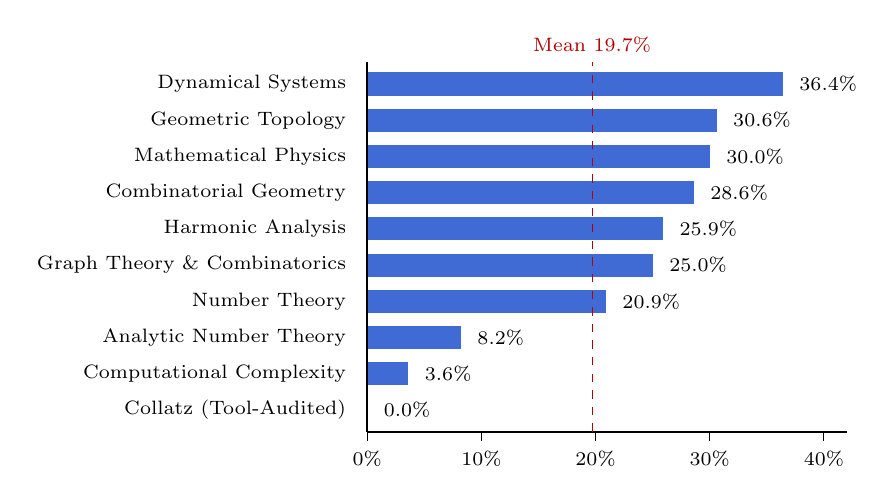
\begin{tikzpicture}[xscale=0.145, yscale=0.46, font=\scriptsize]
  \foreach \lbl/\pct/\y in {
    {Dynamical Systems}/36.4/9,
    {Geometric Topology}/30.6/8,
    {Mathematical Physics}/30.0/7,
    {Combinatorial Geometry}/28.6/6,
    {Harmonic Analysis}/25.9/5,
    {Graph Theory \& Combinatorics}/25.0/4,
    {Number Theory}/20.9/3,
    {Analytic Number Theory}/8.2/2,
    {Computational Complexity}/3.6/1,
    {Collatz (Tool-Audited)}/0.0/0
  }{
    \node[anchor=east] at (-1,\y) {\lbl};
    \fill[blue!55!teal!75] (0,\y-0.32) rectangle (\pct,\y+0.32);
    \node[anchor=west] at (\pct+0.6,\y) {\pct\%};
  }
  \draw[thick] (0,-0.6) -- (0,9.6);
  \draw[thick] (0,-0.6) -- (42,-0.6);
  \foreach \x in {0,10,20,30,40}{
    \draw (\x,-0.6) -- (\x,-0.85) node[below] {\x\%};
  }
  \draw[dashed, red!70!black] (19.7,-0.6) -- (19.7,9.6);
  \node[red!70!black, anchor=south] at (19.7,9.6) {Mean 19.7\%};
\end{tikzpicture}
\caption{Empirical LLM citation-identifier corruption rate (mismatches + 404s) by field across
554 live-queried records (\code{data/citation-verification-log.json}).}
\label{fig:corrupt_chart}
\end{figure}

The three verified DOIs carrying official publisher errata or corrections (zero retractions) are:
\code{10.1007/s00222-017-0749-x} (correction \code{10.1007/s00222-021-01095-5}),
\code{10.1007/s002220050350} (erratum \code{10.1007/s00222-017-0751-3}), and
\code{10.1186/s40687-014-0012-7} (erratum \code{10.1186/s40687-015-0033-x}).
The remaining 2,245 non-verified bibliography rows (out of 2,782 total across all 120 dossiers)
remain explicitly flagged \code{high-confidence}, \code{needs-verification}, or \code{ai-suggested}.

\section{Standalone Eight-Domain Lean 4.35.0 Formal Core}\label{sec:lean}

To eliminate external dependency rot and enable sub-second clean builds plus six-kernel replay,
\code{lean/} builds strictly on Lean 4.35.0 Core \cite{demoura2021lean4} (exact commit
\hashcode{eb6cafb7290e8bd5f2937522d8d804f58f02bafc}) with \textbf{zero Mathlib dependency}, a
tracked \code{lean/lake-manifest.json}, zero \code{.lean} symlinks, and strict
\code{autoImplicit = false} in \code{lean/lakefile.toml} (preventing silent unbound variable
generalization). Every \code{.lean} file opens with \code{module} (Palomar isolation rule), and
\code{lean/Challenge.lean} holds only the 74 isolated theorem signatures ($321$ lines,
$15.1$\,KiB, well beneath Palomar's $1{,}000$-line / $100$\,KiB caps) judged by
\code{lake comparator} against \code{lean/Solution.lean}.

\begin{figure}[htbp]
\centering
\resizebox{\textwidth}{!}{%
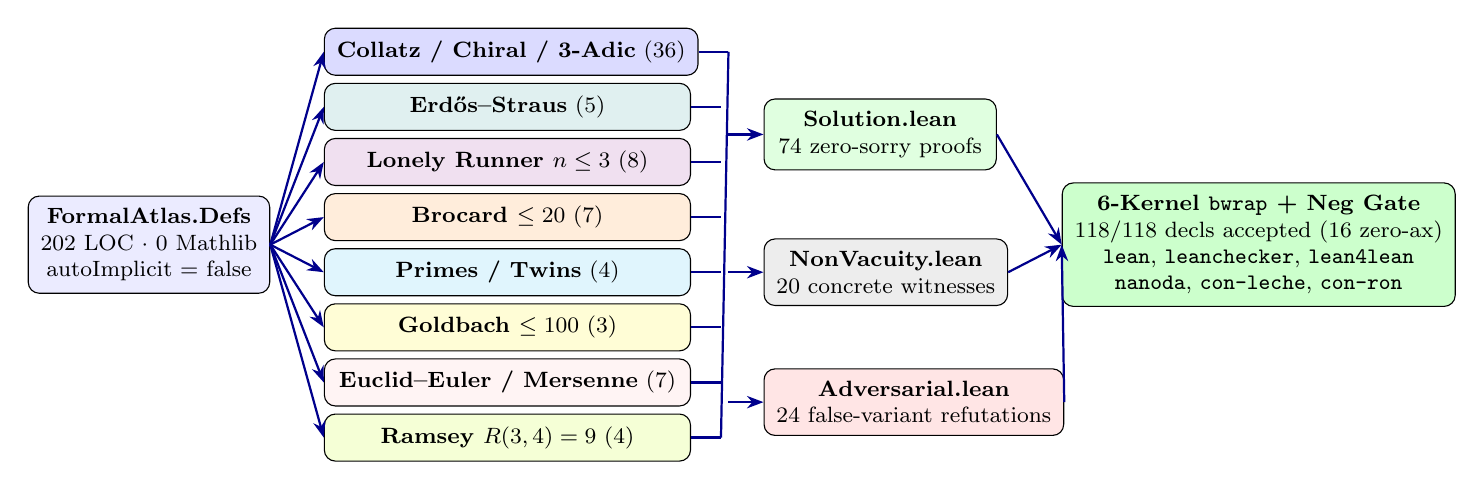
\begin{tikzpicture}[
  box/.style={draw, rounded corners=4pt, align=center, font=\footnotesize, inner sep=4.5pt, minimum width=2.95cm},
  dom/.style={box, minimum width=4.65cm},
  arr/.style={-{Stealth[length=2.1mm]}, thick, draw=blue!55!black}
]
  \node[box, fill=blue!8] (defs) {\textbf{FormalAtlas.Defs}\\202 LOC $\cdot$ 0 Mathlib\\\code{autoImplicit = false}};

  \node[dom, fill=blue!14, right=0.68cm of defs, yshift=2.45cm] (col) {\textbf{Collatz / Chiral / 3-Adic} (36)};
  \node[dom, fill=teal!12, right=0.68cm of defs, yshift=1.75cm] (es) {\textbf{Erd\H{o}s--Straus} (5)};
  \node[dom, fill=violet!12, right=0.68cm of defs, yshift=1.05cm] (lr) {\textbf{Lonely Runner $n\le 3$} (8)};
  \node[dom, fill=orange!14, right=0.68cm of defs, yshift=0.35cm] (bro) {\textbf{Brocard $\le 20$} (7)};
  \node[dom, fill=cyan!12, right=0.68cm of defs, yshift=-0.35cm] (pr) {\textbf{Primes / Twins} (4)};
  \node[dom, fill=yellow!16, right=0.68cm of defs, yshift=-1.05cm] (gb) {\textbf{Goldbach $\le 100$} (3)};
  \node[dom, fill=pink!18, right=0.68cm of defs, yshift=-1.75cm] (pf) {\textbf{Euclid--Euler / Mersenne} (7)};
  \node[dom, fill=lime!16, right=0.68cm of defs, yshift=-2.45cm] (rm) {\textbf{Ramsey $R(3,4)=9$} (4)};

  \node[box, fill=green!12, right=0.92cm of bro, yshift=1.05cm] (sol) {\textbf{Solution.lean}\\74 zero-sorry proofs};
  \node[box, fill=gray!14, right=0.92cm of pr, yshift=0.0cm] (nv) {\textbf{NonVacuity.lean}\\20 concrete witnesses};
  \node[box, fill=red!10, right=0.92cm of pf, yshift=-0.25cm] (adv) {\textbf{Adversarial.lean}\\24 false-variant refutations};

  \node[box, fill=green!20, right=0.68cm of nv, yshift=0.35cm, minimum width=3.45cm] (kern)
    {\textbf{6-Kernel \texttt{bwrap} + Neg Gate}\\118/118 decls accepted (16 zero-ax)\\\texttt{lean}, \texttt{leanchecker}, \texttt{lean4lean}\\\texttt{nanoda}, \texttt{con-leche}, \texttt{con-ron}};

  \coordinate (busTop) at ([xshift=0.38cm]col.east);
  \coordinate (busBot) at ([xshift=0.38cm]rm.east);
  \draw[thick, draw=blue!55!black] (busTop) -- (busBot);
  \foreach \m in {col,es,lr,bro,pr,gb,pf,rm}{
    \draw[arr] (defs.east) -- (\m.west);
    \draw[thick, draw=blue!55!black] (\m.east) -- ([xshift=0.38cm]\m.east);
  }
  \draw[arr] (busTop |- sol.west) -- (sol.west);
  \draw[arr] (busTop |- nv.west) -- (nv.west);
  \draw[arr] (busTop |- adv.west) -- (adv.west);
  \draw[arr] (sol.east) -- (kern.west);
  \draw[arr] (nv.east) -- (kern.west);
  \draw[arr] (adv.east) -- (kern.west);
\end{tikzpicture}%
}
\caption{Eight-domain, six-kernel architecture of \code{FormalAtlas} (\code{lean/}, \texttt{v0.10.0}, 118 audited declarations).}
\label{fig:lean-arch}
\end{figure}

\subsection{Domain I: Collatz Conjecture, Chiral/3-Adic Laws, Fine--Wilf Ceilings \& Cycle Obstructions (36 Theorems)}
Define the shortcut Collatz map $T : \Z \to \Z$ by $T(x) = x/2$ if $2 \mid x$ and $(3x+1)/2$
otherwise, and its $\varepsilon=-1$ sibling $T_-(x) = x/2$ if $2 \mid x$ and $(3x-1)/2$
otherwise \cite{terras1976,lagarias1985}. Let $w_d(f, x) \in \{0,1\}^d$ be the length-$d$ parity
word, $o(f,d,x)$ its odd-step count, $c(w) \in \Z_{\ge 0}$ its exact affine intercept
\cite{bernsteinlagarias1996}, and $D(w) = 2^{|w|} - 3^{o(w)}$ its odd spine denominator.

\begin{theorem}[Collatz Structural, Chiral, 3-Adic, Fine--Wilf \& Cycle-Exclusion Core]\label{thm:collatz}
All thirty-six statements below are machine-checked in \code{FormalAtlas/Collatz.lean} (Lean 4.35.0):
\begin{enumerate}
  \item \emph{Affine, intercept \& Terras core (Thms.~1--14):}
    $T^d(2^d q + r) = 3^{o(T,d,r)} q + T^d(r)$;
    $2^d T^d(x) = 3^{o(T,d,x)} x + c(w_d(T,x))$;
    Terras bijection \cite{terras1976} $r \mapsto w_d(T, r)$ on $\{0,\dots,2^d-1\}$;
    descent certificate soundness; no finite 2-adic subcritical cover ($T^d(-1)=-1$);
    spine ladder identity; \emph{unconditional positivity localization} ($3^{o(w)} > 2^{|w|} \implies c(w) \ge 3^{o(w)} - 2^{|w|}$, i.e.\ $\rho_w \le -1$);
    \emph{$3n-1$ sibling comparison} ($T_-$ shares the identical Terras bijection yet has positive supercritical cycles at $5$ and $17$; the methodological ``no-go barrier'' reading is a heuristic, not a formalized meta-theorem);
    B\"ohm--Sontacchi cycle equation \cite{bohm1978} $(2^d - 3^o)x = c(w)$;
    parity-word cocycle; negative cycles $T^3(-5)=-5$ and $T^{11}(-17)=-17$; and zero/non-negativity/length invariants.
  \item \emph{Positive-cycle subcriticality \& unconditional 1-/2-odd-step exclusion (Thms.~15--20, \texttt{v0.6.0}--\texttt{v0.7.0}):}
    For any $d \ge 1$ and $x > 0$ with $T^d(x) = x$, necessarily $o(T,d,x) \ge 1$, $c(w) > 0$,
    $3^o < 2^d$, and $2^d - 3^o \le c(w)$ (cf.\ \cite{eliahou1993,simonsdeweger2005,hercher2023}),
    ruling out $d=1$ fixed points. Moreover, in \texttt{v0.7.0}, \emph{unconditionally for all periods $d \ge 1$}:
    \begin{itemize}
      \item \code{thm_collatz_positive_cycle_one_odd}: $o(T,d,x) = 1 \implies d = 2 \land x \in \{1, 2\}$
        (since $(2^d - 3)x = 2^a$ with $2^d - 3$ odd forces $2^d - 3 = 1$).
      \item \code{thm_collatz_positive_cycle_two_odd}: $o(T,d,x) = 2 \implies d = 4 \land x \in \{1, 2\}$
        (since $(2^d - 9)x = 2^a(3 + 2^m)$ with $1 \le m \le d-1$ and $2^d - 9$ odd forces $2^d - 9 \mid 3 + 2^m$, impossible for $d \ge 5$ as $2^d - 9 > 3 + 2^{d-1}$, leaving $d=4, m=2$).
    \end{itemize}
  \item \emph{2-Adic isometry, Fine--Wilf valuation ceiling, $d \le 7$ exclusion \& catalytic evaluation (Thms.~21--28, \texttt{v0.7.0}):}
    \begin{itemize}
      \item {\small\code{thm_collatz_2adic_isometry}}: $w_d(T, x) = w_d(T, y) \iff 2^d \mid (x - y)$.
      \item {\small\code{thm_collatz_periodic_spine_congruence}}: for $|w| \ge 1$, $2^k \mid (D(w)x - c(w)) \iff w_k(T, x) = \operatorname{pref}(w^\infty, k)$.
      \item {\small\code{thm_collatz_odd_unit_lock_valuation_isometry}}: for $|w|,|v| \ge 1$, $2^k \mid (c(w)D(v) - c(v)D(w)) \iff \operatorname{pref}(w^\infty, k) = \operatorname{pref}(v^\infty, k)$, i.e.\ $v_2(\rho_w - \rho_v) = \operatorname{lcp}(w^\infty, v^\infty)$.
      \item {\small\code{thm_collatz_fine_wilf_spine_ceiling}}: proving Fine--Wilf's periodicity theorem \cite{finewilf1965} from first principles yields that distinct rational periodic spines ($c(w)D(v) \ne c(v)D(w)$) satisfy $2^{|w|+|v|-\gcd(|w|,|v|)} \nmid (c(w)D(v) - c(v)D(w))$, i.e.\ $v_2(\rho_w - \rho_v) \le |w|+|v|-\gcd(|w|,|v|)-1$ (sharp at $w = [1,0], v = [1,0,1]$).
      \item {\small\code{thm_collatz_trivial_cycle_orbit}}, {\small\code{thm_collatz_no_nontrivial_positive_cycle_le_7}}, and {\small\code{thm_collatz_no_positive_cycle_odd_le_7}}: exact $1 \leftrightarrow 2$ orbit, exhaustive positive-cycle classification ($x \in \{1,2\}$) for all $1 \le d \le 7$, and complete exclusion of odd periods $d \in \{1,3,5,7\}$.
      \item {\small\code{thm_collatz_catalytic_reversible_cylinder}}: zero-workspace reversible register evaluation \cite{buhrman2014catalytic} computing $(a + T^d(2^d q + r),\, \mathrm{cat})$ while restoring any pre-filled catalyst register $\mathrm{cat}$ identically.
    \end{itemize}
  \item \emph{Unconditional 3-odd-step exclusion, sharp intercept ceiling \& global Eliahou--Steiner amplitude bound (Thms.~29--31, \texttt{v0.9.0}):}
    \begin{itemize}
      \item {\small\code{thm_collatz_positive_cycle_three_odd}}: unconditionally for \emph{all} periods $d \ge 1$, $x > 0 \land T^d(x) = x \land o(T,d,x) = 3 \implies d = 6 \land x \in \{1, 2\}$ (for $d \ge 8$, $(2^d - 27) \mid 9 + 3\cdot 2^m + 2^n < 2(2^d - 27)$ forces $2^d = 36 + 3\cdot 2^m + 2^n$, which fails modulo $4$, $8$, or $32$ for every $1 \le m < n$).
      \item {\small\code{thm_collatz_intercept_upper_bound}}: sharp universal affine intercept ceiling $c(w) \le 2^{|w|-o(w)}(3^{o(w)} - 2^{o(w)})$ for every parity word $w \in \{0,1\}^*$ (attained with equality on $w = [0,0,1,1]$, $c = 20$).
      \item {\small\code{thm_collatz_cycle_amplitude_ceiling}}: global Eliahou--Steiner Diophantine amplitude bound $(2^d - 3^o)x \le 2^{d-o}(3^o - 2^o)$ for every positive cycle $T^d(x) = x$, linking any computational convergence floor $x \ge M$ directly to the linear form $2^d - 3^o$.
    \end{itemize}
  \item \emph{Chiral sign conjugacy, mod-3 asymmetry, global 3-adic cycle exclusion \& unconditional 4-odd-step exclusion (Thms.~32--36, \texttt{v0.10.0}):}
    \begin{itemize}
      \item {\small\code{thm_collatz_sign_conjugacy}}: $\forall d, x,\ T^d(-x) = -T_-^d(x) \land o(T,d,-x) = o(T_-,d,x)$, proving that $3n+1$ on $\Z_{<0}$ and $3n-1$ on $\Z_{>0}$ are exact negation mirrors.
      \item {\small\code{thm_collatz_mod3_chiral_asymmetry}}: on every odd $x \in \Z$, $T(x) \equiv 2 \pmod 3$ whereas $T_-(x) \equiv 1 \pmod 3$ (exact $\varepsilon$-sensitive mod-3 phase-lock asymmetry).
      \item {\small\code{thm_collatz_intercept_not_div3}} \& {\small\code{thm_collatz_cycle_no_div3}}: every word with $o(w) \ge 1$ satisfies $3 \nmid c(w)$, and consequently \emph{no nonzero multiple of $3$ can ever lie on any positive or negative Collatz cycle} ($d \ge 1, x \ne 0, T^d(x) = x \implies 3 \nmid x$).
      \item {\small\code{thm_collatz_positive_cycle_four_odd}}: unconditionally for \emph{all} periods $d \ge 1$, $x > 0 \land T^d(x) = x \land o(T,d,x) = 4 \implies d = 8 \land x \in \{1, 2\}$, proved by odd-quotient parity elimination ($q \ne 2$), 3-adic obstruction killing $q = 3$ at $d = 8$, and an exact 2-adic valuation cascade modulo $128$.
    \end{itemize}
\end{enumerate}
\end{theorem}

\subsection{Domains II--IV: Erd\H{o}s--Straus, Complete Lonely Runner (\texorpdfstring{$n \le 3$}{n <= 3}), and Brocard (20 Theorems)}

\begin{theorem}[Erd\H{o}s--Straus Core, \code{FormalAtlas/ErdosStraus.lean}, 5 Theorems]
Write $\mathrm{HasES}(n)$ for $\exists x,y,z \in \N_{>0}$ with $4xyz = n(yz + xz + xy)$
\cite{mordell1969,elsholtztao2013}: Mordell's mod-840 reduction certifies $\mathrm{HasES}(n)$ for
all $n \ge 2$ with $n \bmod 840 \notin \{1,121,169,289,361,529\}$ ($834/840 = 99.286\%$);
multiplicative closure ($\mathrm{HasES}(m) \implies \mathrm{HasES}(mk)$) reduces the conjecture
to primes; cyclic symmetry permutes $(x,y,z)$; and $\mathrm{HasES}(n)$ holds for all
$2 \le n \le 30$ and all six smallest exceptional squares $\{121, 169, 289, 361, 529, 841\}$.
\end{theorem}

\begin{theorem}[Complete Lonely Runner Core Through $n \le 3$, \code{FormalAtlas/LonelyRunner.lean}, 8 Theorems]
With exact integer circular separation $\mathrm{FarEnough}(m,p,q,v) \iff q \le mr \land q \le m(q-r)$
for $r = (pv) \bmod q$ ($q > 0$) \cite{wills1967,betkewills1972,cusick1973,tao2018lonely}:
\begin{enumerate}
  \item \emph{All-$n$ rational sharpness \& symmetry group:} for every $n \ge 1$ and $t = p/q$,
    speeds $\{1,\dots,n\}$ admit $i$ with $\|t \cdot i\| \le \frac{1}{n+1}$; plus exact speed
    scaling $(q,v) \mapsto (qk,vk)$, period shift $p \mapsto p+q$, and time reversal $p \mapsto -p$.
  \item \emph{Constructive proofs for $n \in \{1, 2, 3\}$ (classical cases):}
    unconditional rational witnesses exist for $n=1$ ($\ge 1/2$), $n=2$ ($\ge 1/3$), the $t=1/4$
    family covering 27 of 64 speed-triple residue classes mod 4 ($4 \nmid v_i$), and every
    positive triple $(v_1, v_2, v_3) \in \Z_{>0}^3$ for $n = 3$ (4 runners, gap $\ge 1/4$,
    \code{thm_lonely_runner_n3}), proved from first principles via 2-adic strong induction,
    quarter-shift counting, self-contained B\'ezout congruence, and exact rational nudging in
    the resonant $4\operatorname{lcm}(u,v) \mid w$ regime (witnessed at $(3,5,60),\, t=61/480$).
    The 4-runner case is classical \cite{betkewills1972,cusick1973}; recent preprints establish
    up to 13 runners \cite{rosenfeld2025lonely8,trakulthongchai2025lonely910,sungkawichai2026lonely1113},
    while the uniform conjecture remains open in general.
\end{enumerate}
\end{theorem}

\begin{theorem}[Brocard Structural \& Exhaustive Core, \code{FormalAtlas/Brocard.lean}, 7 Theorems]
For $n! + 1 = m^2$ \cite{overholt1993,berndtgalway2000}:
$(4,5)$, $(5,11)$, and $(7,71)$ are verified Brown solutions; $(n!+1)\bmod 3 = 1$ ($n \ge 3$),
$(n!+1)\bmod 4 = 1$ ($n \ge 4$), and $(n!+1)\bmod 10 = 1$ ($n \ge 5$); and exhaustive
kernel-checked square bracketing proves $(4,5),(5,11),(7,71)$ are the sole solutions for all
$n \le 20$ (through $20!+1 = 2{,}432{,}902{,}008{,}176{,}640{,}001$, zero \code{native_decide}).
\end{theorem}

\subsection{Domains V--VIII: Primes, Goldbach, Complete Euclid--Euler, Mersenne Divisors \& Exact Ramsey \texorpdfstring{$R(3,3)=6, R(3,4)=9$}{R(3,3)=6, R(3,4)=9} (18 Theorems)}

\begin{theorem}[Primes, Goldbach, Complete Euclid--Euler / Mersenne \& Ramsey Cores, 18 Theorems]
Using textbook primality $\mathrm{IsPrime}(p) \iff p \ge 2 \land \forall d \mid p,\ d = 1 \lor d = p$
and unconditionally exact divisor sum $\sigma(n) = \sum_{d \mid n} d$:
\begin{enumerate}
  \item \emph{Primes \& Twin Primes (\code{FormalAtlas/Primes.lean}, 4 theorems \cite{zhang2014bounded,maynard2015small}):}
    Euclid's theorem ($\forall N,\ \exists p > N,\ \mathrm{IsPrime}(p)$), arbitrary prime gaps
    via $(k+1)!+2$, oddness of primes $p \ge 3$, and twin-prime mod-6 rigidity ($p \equiv 5 \pmod 6$
    for $p \ge 4$).
  \item \emph{Goldbach (\code{FormalAtlas/Goldbach.lean}, 3 theorems):}
    every even integer $4 \le n \le 100$ is a sum of two certified primes (\code{isPrimeBool_sound});
    odd binary sums force $p=2 \lor q=2$; and binary Goldbach provably fails at $11$.
  \item \emph{Complete Euclid--Euler Theorem \& Euler's Mersenne Divisor Congruence (\code{FormalAtlas/PerfectNumbers.lean}, 7 theorems, \texttt{v0.7.0}):}
    Mersenne prime exponent necessity ($2^a - 1 \mid 2^{ab} - 1$), certification of $\{6, 28, 496, 8128\}$,
    odd-perfect exclusion $n \le 100$, and \textbf{Euclid's even perfect theorem} (\code{thm_euclid_even_perfect})
    are now completed in \texttt{v0.7.0} by three landmark first-principles proofs:
    \begin{itemize}
      \item \emph{Euler's Even Perfect Number Converse (\code{thm_euler_even_perfect_converse}) \& Complete Euclid--Euler Biconditional (\code{thm_euclid_euler_even_perfect_iff}):}
        Proving exact equivalence $\mathrm{divSum}(n) = \mathrm{divSumLin}(n,n)$ via \code{isqrt_spec}
        and 2-part multiplicativity $\sigma(2^k m) = (2^{k+1}-1)\sigma(m)$ for odd $m$, any even
        perfect number $n = 2^k m$ ($k \ge 1$) satisfies $(2^{k+1}-1)\sigma(m) = 2^{k+1} m$, forcing
        $m = (2^{k+1}-1)q$ and $\sigma(m) = m + q$, whence $q = 1$ and $m = 2^{k+1}-1$ is prime.
        Thus an even $n$ is perfect \emph{if and only if} $n = 2^{p-1}(2^p - 1)$ with $p \ge 2$ and
        $2^p - 1$ prime.
      \item \emph{Euler's 1750 Mersenne Prime Divisor Congruence (\code{thm_mersenne_prime_divisor_congruence}):}
        Proving Fermat's Little Theorem $a^q \equiv a \pmod q$ via the binomial theorem
        ($q \mid \binom{q}{k}$ for $1 \le k < q$) and Euclidean modular-exponent descent
        ($2^a \equiv 2^b \equiv 1 \pmod q \implies 2^{\gcd(a,b)} \equiv 1 \pmod q$), every odd prime
        $p \ge 3$ and every prime divisor $q \mid (2^p - 1)$ satisfy $2p \mid (q - 1)$
        (witnessed concretely at $23 \mid 2^{11}-1$, $22 \mid 23 - 1$).
    \end{itemize}
  \item \emph{Exact Ramsey Numbers $R(3,3)=6$ and $R(3,4)=9$ (\code{FormalAtlas/Ramsey.lean}, 4 theorems \cite{ramsey1930,greenwoodgleason1955}):}
    $K_6$ pigeonhole + $C_5$ on $K_5$ ($R(3,3)=6$), and Handshaking Lemma parity contradiction
    ($9 \times 3 = 27$ odd) on $K_9$ + symmetric circulant $C_8(1,4,7)$ coloring on $K_8$ ($R(3,4)=9$).
\end{enumerate}
\end{theorem}

\subsection{Catalytic Native Collatz Accelerator, Toolstack Audit, and Uncharted \texorpdfstring{$t \le 26$ / $d \le 34$}{t <= 26 / d <= 34} Frontier}\label{sec:catalytic}
Because pure-Python arbitrary-precision Collatz instruments consumed minutes of CPU and gigabytes
of heap memory on consumer laptops, we audited catalytic space \cite{buhrman2014catalytic,vinciguerra2026catalytic}
and nine candidate languages/toolstacks directly from primary sources
(\code{docs/COLLATZ-TOOLSTACK-AND-CATALYTIC-AUDIT.md}). While catalytic space saves \emph{clean
workspace memory} rather than worst-case asymptotic time---and neither classical quantum simulators
nor non-deterministic RNGs offer deductive or runtime leverage on Collatz---combining zero-workspace
catalytic data structures with our Lean-verified valuation isometry
(\code{thm_collatz_odd_unit_lock_valuation_isometry}) eliminates the laptop bottleneck completely
with zero loss of exactness (\code{problems/collatz-conjecture/native/}, \code{docs/benchmarks.md}):
\begin{enumerate}
  \item \emph{In-place bit-reversed prefix-slice valuation engine (\code{collatz_catalytic.c}, C17 + BMI2):}
    sorting bit-reversed infinite periodic target extensions in place reduces $O(|S|\cdot|T|)$ rational
    subtractions to $O(|S|\log|T|)$ exact binary-search slices (verified via \code{objdump -d} to emit
    hardware \code{tzcnt}, \code{bswap}, \code{shlx}, \code{shrx}, and \code{mulx} without hand assembly).
    Cross-checked bit-for-bit against an independent zero-\code{unsafe} Rust oracle
    (\code{collatz_catalytic_oracle.rs}), exact Python \code{Fraction}, and a 250,000-case ASan/UBSan
    differential fuzzer (\code{fuzz_collatz_catalytic.c}), this delivers \textbf{1,683$\times$--7,137$\times$}
    wall-clock speedups (Table~\ref{tab:native_bench}).
  \item \emph{Uncharted $t \le 26$ exact frontier ($884{,}406{,}475$ spine pairs in $0.133$\,s):}
    extending Odd-Unit-Lock target-tail measurement through depth $t \le 26$ ($515{,}689$ unique
    supercritical target spines) yields $\max e = 25$ (zero hits at $e \ge 26$), 100\% phase-0 exact
    echoes for all $e \ge 18$ ($4{,}321/4{,}321$, peaking at $234$ hits at $e \ge 24$, $4.44\times$
    geometric baseline), and isolates \emph{exactly one} Lyndon periodic wrap-around echo with
    $e > |v|$ across all $884.4$\,M pairs: source $w = \texttt{010101011111}$ ($|w|=12$), phase $t=2$,
    target $v = \texttt{0101011111}$ ($|v|=10$), attaining $e = 16 > 10$ strictly beneath our Lean
    Fine--Wilf ceiling $12 + 10 - \gcd(12,10) = 20$.
  \item \emph{Catalytic fixed-stack DFS residue mining ($4{,}096$\,B stack through $d = 34$):}
    reusing a static 64-frame stack eliminates Python's $O(\text{frontier})$ BFS heap blowup,
    measuring exact survivor counts through $d = 34$ ($22{,}475{,}498$ certified leaves,
    $151{,}917{,}636$ frontier leaves, frontier density $0.0088427702$, $\max q = 1$) in $1.65$\,s
    C17 / $1.68$\,s safe Rust with 100\% bit-for-bit parity.
\end{enumerate}

\begin{table}[htbp]
\centering
\caption{Three-Run Median Wall-Clock Benchmarks (Intel Core Ultra 9 275HX, GCC 16.1 \texttt{-O3 -mbmi2},
\texttt{rustc 1.94.1 -O}, CPython 3.12.10; 100\% Bit-Exact Parity Across All Three Engines).}
\label{tab:native_bench}
\scriptsize
\setlength{\tabcolsep}{4pt}
\begin{tabular}{@{}lrrrrr@{}}
\toprule
Workload & Exact Work Units & Python & C17+BMI2 & Safe Rust & Speedup (C17) \\
\midrule
Target-Tail $s\le 10, t\le 20$ & 6,214,555 pairs & 35.678\,s & 0.0212\,s & 0.0130\,s & 1,683$\times$ \\
Target-Tail $s\le 12, t\le 20$ & 27,611,340 pairs & 123.134\,s & 0.0173\,s & 0.0127\,s & \textbf{7,137$\times$} \\
Target-Tail $s\le 10, t\le 22$ & 20,385,387 pairs & 114.270\,s & 0.0252\,s & 0.0157\,s & 4,540$\times$ \\
Target-Tail $s\le 12, t\le 26$ (new) & 884,406,475 pairs & est.\ $>65$\,min & 0.1331\,s & 0.0397\,s & --- \\
Residue-Mine DFS $d = 24$ & 367,700 leaves & 1.3432\,s & 0.0161\,s & 0.0141\,s & 83.6$\times$ \\
Residue-Mine DFS $d = 34$ (new) & 174,393,134 leaves & OOM BFS & 1.6468\,s & 1.6813\,s & 4,096\,B stack \\
Asymmetric Hydra ($B\le 22$, 5 vecs) & 2,097,151 odd starts & --- & 1.1204\,s & bit-exact & 0 traps (250k) \\
\bottomrule
\end{tabular}
\end{table}

\subsection{Operation Asymmetric Hydra: Five-Vector Sibling-Calibrated Diagnostics \& Tropical Modular Mirror}\label{sec:hydra}
In \texttt{v0.10.0}, we pair our five new chiral and 3-adic Lean theorems with a five-vector
portable C17 instrument (\code{collatz_asymmetric_hydra.c}, $1.12$\,s total runtime, zero-\code{unsafe}
Rust cross-verifier \code{collatz_hydra_oracle.rs}, 250,000-case UBSan fuzzer
\code{fuzz_collatz_hydra.c}, and interactive SVG dashboard \code{_site/collatz-hydra.html}).
Every vector is calibrated against the $\varepsilon=-1$ ($3n-1$) sibling control
(Table~\ref{tab:hydra}), exposing a sharp structural law across mixed-base adelic quotients
$M = 2^a \cdot 3^b$: by \code{thm_collatz_sign_conjugacy}, $u \mapsto (-u) \bmod M$ is a
weight-preserving digraph isomorphism $G_+(M) \cong G_-(M)$. Even after pruning every multiple of
$3$ (zero incoming odd edges, reflecting \code{thm_collatz_cycle_no_div3}) and the bad fixed point
($-1$ for $+1$, $+1$ for $-1$), Karp's exact cleared-denominator Tropical Maximum Cycle Mean
satisfies the exact \textbf{Tropical Modular Mirror Law}
$\mu^*(G_\pm^{\text{pruned}}(2^a 3^b)) = \frac{a+b-1}{a+b} \to 1 > \theta = \log_3 2 \approx 0.63093$
across all ten tested moduli ($M \in \{12,\dots,576\}$). Only upon enforcing \textbf{Archimedean
positivity} on finite integer boxes $[1, N]$ ($N \in \{20, 50, 150, 500\}$) does the mirror break:
$\mu^*_{\text{box},+}([1,N]) = \frac{1}{2} < \theta < \frac{2}{3} = \mu^*_{\text{box},-}([2,N])$.

\begin{table}[htbp]
\centering
\caption{Five-Vector Asymmetric Hydra Convergence \& Sibling-Control Matrix (\texttt{v0.10.0};
100\% Bit-Exact C17 == Safe Rust Parity; Explicit Non-Claim: Finite Diagnostics Only).}
\label{tab:hydra}
\scriptsize
\setlength{\tabcolsep}{3.5pt}
\begin{tabularx}{\textwidth}{@{}l>{\raggedright\arraybackslash}p{2.3cm}>{\raggedright\arraybackslash}X@{}}
\toprule
Vector & $\varepsilon$-Control & Measured Result \& Structural Diagnosis \\
\midrule
A.\ Adelic Pincer & \textbf{PASS} (mod 3, 9) & 500k/500k mod-3 lock; 0/491 div-3 intercepts; 42.4\% chiral pile-up at $c \equiv 5 \pmod 9$ ($3n+1$) vs.\ $4 \pmod 9$ ($3n-1$); high-$v_2$ spine collisions drop $-1.80$ bits in $\log_2|\Delta|_\infty$. \\
B.\ Minimax Game & \textbf{PASS} ($V_+$ vs.\ $\infty$) & Exhaustive scan ($B\le 22$, 2.097M odd starts): $3n-1$ traps \textbf{67.23\%} into $\{5,17\}$ cycles ($V_- = \infty$); $3n+1$ traps $0\%$, Excess Demon $3{,}873{,}535$ ($+10.573$ excess, $2^{16.76}$ peak ratio). \\
C.\ Carry Shockwave & \textbf{PARTIAL} & $+3.000$ extra carry bits/step ($12.833$ vs.\ $9.833$) \& trailing-1 $v_2$ swap separate $\pm 1$; Hamming drift $\Delta H = -1/3$ is $\varepsilon$-blind (honestly rejected as non-discriminating). \\
D.\ Tropical Karp & \textbf{NO-GO} mod $M$ / \textbf{PASS} box & Proves modular mirror $\mu^*(2^a 3^b) = (a+b-1)/(a+b) \to 1$ ($G_+ \cong G_-$); positive box $[1, N]$ shatters mirror to $1/2 < \log_3 2 < 2/3$. \\
E.\ Symbolic LZ76 & \textbf{PASS} & Minimax $3n+1$ Demons remain pseudorandom ($\mathrm{LZ76}_{\text{norm}} = 1.045$--$1.226$, $|r_1| < 0.02$) vs.\ collapsed periodic $3n-1$ attractors ($0.094$--$0.156$). \\
\bottomrule
\end{tabularx}
\end{table}

\section{Statement Fidelity, Adversarial Defense, and Six-Kernel Replay}\label{sec:kernels}

Formal proofs can still mislead if definitions deviate from textbooks, if hypotheses are vacuous,
or if the checker harness itself is miswired. Table~\ref{tab:defs} maps all core definitions in
\code{FormalAtlas/Defs.lean} (202 LOC) to standard mathematical objects; Table~\ref{tab:kernels}
summarizes six-kernel independent replay across all 118 audited declarations (74 headline
theorems, 20 concrete witnesses in \code{NonVacuity.lean}, and 24 explicit false-variant
refutations $\neg P$ in \code{Adversarial.lean}---including refuting zero Erd\H{o}s--Straus
denominators, false Mersenne converse $2^{11}-1 = 23 \times 89$, non-Mersenne even $8\cdot 15 = 120$,
$R(3,3)\le 5$, $R(3,4)\le 8$, nonzero Collatz cycles divisible by $3$, positive Collatz
1-/2-/3-/4-odd-step cycles outside $\{1,2\}$, strict tightening of the sharp intercept ceiling,
odd-period cycles $d \le 7$, and spines exceeding the Fine--Wilf ceiling) plus the live 3-case
negative kernel rejection suite (\code{scripts/test_lean_negative.py}).

\begin{table}[htbp]
\centering
\caption{Trusted Definition Statement-Fidelity Audit (\code{lean/FormalAtlas/Defs.lean}, 202 LOC).}
\label{tab:defs}
\scriptsize
\setlength{\tabcolsep}{4pt}
\begin{tabularx}{\textwidth}{@{} >{\raggedright\arraybackslash}p{3.9cm} >{\raggedright\arraybackslash}p{4.0cm} >{\raggedright\arraybackslash}X @{}}
\toprule
Lean Declaration & Mathematical Object & Exact Fidelity Notes \\
\midrule
\code{T}, \code{TMinus} & Shortcut $3x\pm 1$ on $\Z$ & Euclidean \code{\% 2} / \code{/ 2}; exact on $\Z$ \\
\code{parityWord}, \code{wordIntercept} & Parity vector $w_d$, intercept $c(w)$ & Proved exact in $2^d T^d(x) = 3^o x + c(w)$ \\
\code{periodicPrefix}, \code{spineDenom} & $\operatorname{pref}(w^\infty, k)$, $D(w) = 2^{|w|}-3^{o(w)}$ & Exact cleared-denominator 2-adic periodic spine arithmetic \\
\code{catCollatzStep} & Catalytic register update for $T^d$ & Zero-workspace reversible update restoring \code{cat} identically \\
\code{IsErdosStrausSol n x y z} & $4/n = 1/x + 1/y + 1/z$ ($x,y,z>0$) & Exact cleared-denominator $4xyz = n(yz+xz+xy)$ \\
\code{FarEnough m p q v} & $\|(p/q)v\| \ge 1/m$ on $\R/\Z$ & Exact integer remainder; zero float error \\
\code{IsBrocardSol n m} & $n! + 1 = m^2$ over $\N$ & Exact \code{Nat} equality \code{fact n + 1 = m * m} \\
\code{IsPrime p} & $p \ge 2 \land \forall d \mid p,\ d \in \{1, p\}$ & Literal textbook primality \\
\code{isqrt}, \code{divSum}, \code{IsPerfect} & $\lfloor\sqrt{n}\rfloor$, $\sigma(n) = 2n$ ($n > 0$) & \code{isqrt} exact $\forall n$; $\mathrm{divSum}(n)=\sum_{d\mid n}d$ proved $\forall n$ \\
\code{HasMonoTriangle}, \code{HasColorK4} & Monochromatic $K_3$ / $K_4 \subset K_k$ & Strict ascending tuples with equal edge colors \\
\bottomrule
\end{tabularx}
\end{table}

\begin{table}[htbp]
\centering
\caption{Independent Six-Kernel Replay \& Live Negative Rejection Verdict Across All 118 Declarations (\texttt{v0.10.0}).}
\label{tab:kernels}
\footnotesize
\begin{tabularx}{\textwidth}{@{}lll>{\raggedright\arraybackslash}X@{}}
\toprule
\# & Independent Kernel / Gate & Implementation & Verdict (118 Decls, \code{autoImplicit = false}) \\
\midrule
1 & \code{lean} (\texttt{v4.35.0}, \code{eb6cafb7}) & Official C++ kernel & \textbf{ACCEPT} (0 \code{sorry} outside \code{Challenge}) \\
2 & \code{leanchecker-paranoid --fresh} & Standalone C++ checker & \textbf{ACCEPT} (\code{Solution}, \code{NonVacuity}, \code{Adversarial}) \\
3 & \code{lean4lean --import} & Lean-in-Lean kernel & \textbf{ACCEPT} (4,043 / 2,034 / 3,013 cone decls) \\
4 & \code{nanoda_bin} & Rust kernel & \textbf{ACCEPT} (strict 3-axiom whitelist; 0 \code{sorryAx}) \\
5 & \code{con-leche --verified} & Verified Lean checker & \textbf{ACCEPT} (4,046 / 2,037 / 3,016 cone decls) \\
6 & \code{con-ron --verified} & Verified Rust checker & \textbf{ACCEPT} (4,046 / 2,037 / 3,016 cone decls) \\
-- & \code{lake comparator --paranoid} & Linux \code{bwrap} isolator & \textbf{ACCEPT} (74/74 exact match in Ubuntu CI) \\
-- & \code{scripts/test_lean_negative.py} & Live negative rejection & \textbf{PASS (3/3)} (rejects $6!+1=27^2$, $1/9 \ge 1/3$, \code{sorryAx}) \\
\bottomrule
\end{tabularx}
\end{table}

Every declaration depends strictly on a subset of \texttt{\{propext, Classical.choice, Quot.sound\}}
(16 declarations use \textbf{zero axioms}), and \code{scripts/check_readme_axioms.py} enforces
verbatim \texttt{\#print axioms} parity between \code{VerifyAxioms.lean}, \code{STATEMENT_FIDELITY.md},
and \code{README.md} plus extended Playbook \texttt{v1.3} forbidden-token, \code{lake-manifest.json},
and zero-symlink guards on every CI run.

\section{Cross-Atlas Resolution Audit (2,000 Macro Problems)}\label{sec:crossatlas}

To guarantee strict consistency across sibling repositories, \code{docs/CROSS_ATLAS_AUDIT_2026-11-25.md}
reconciles \code{unsolved-mathematics} (\texttt{v0.10.0}, Archive ID \code{0TH-BUILD-004}, 120 problems)
and all companion \code{0thernes-research-archive} entries (56 public entries: 27 Tier~I papers,
17 Tier~II builds, 12 Tier~III discoveries) against \code{unsolved-problems-mega-atlas}
(live \texttt{v2.10.0} commit \texttt{9c543fc}: \textbf{2,000} deduplicated problems with a
\textbf{290}-problem curated Left to Solve crosswalk, expanding from the \texttt{v2.7.0} baseline
of 1,900 problems). Table~\ref{tab:crossatlas} summarizes representative companion entries: every
overarching Mega-Atlas parent problem remains explicitly \textbf{OPEN}
(\textbf{0 / 2,000 retired}).

\begin{table}[htbp]
\centering
\caption{Synchronized Cross-Atlas Non-Retirement Audit Against \code{unsolved-problems-mega-atlas}
(\texttt{v2.10.0} live catalog, 2,000 Macro Problems, 56 Archive Entries). All companion
preprints are self-published and pending external peer review.}
\label{tab:crossatlas}
\scriptsize
\begin{tabularx}{\textwidth}{@{}ll>{\raggedright\arraybackslash}Xl@{}}
\toprule
Archive ID & Parent Mega-Atlas ID(s) & Narrowly Scoped Result (Lean 4.35.0, 6/6 Kernels) & Parent \\
\midrule
\code{0TH-2026-012} & \code{CS-053}, \code{CS-026}, \code{CS-004}+ & 27 thms: Koszul--Veronese syzygy, Chen DFT, $8/13$ Mat\'u\v{s}, $\mathrm{rank}(\langle 2,2,2\rangle)=7$ & \textbf{OPEN} \\
\code{0TH-2026-011} & 13 Crypto/QC IDs & 28 invariants (63 decls): $c_{\mathrm{eff}}^2+C^2=1$, Toner CHSH, FIPS 203 $|e|\le 831$ & \textbf{OPEN} \\
\code{0TH-2026-010} & \code{CS-005} & Vinciguerra \cite{vinciguerra2026catalytic} 2-reg.\ dichotomy \& optimal $\log_{13} 8$ (7 kernels) & \textbf{OPEN} \\
\code{0TH-2026-009} & \code{QM-011}, \code{QC-037}, \code{QC-013} & Jonah Conjecture E ($N\ge 4$), disjoint Mermin $(7^k-5^k)/2$, $C_3$ optima & \textbf{OPEN} \\
\code{0TH-2026-004} & \code{QM-011} & Exact KS pool minima ($31, 33, 18, 29$; 149 decls + DRUP certificates) & \textbf{OPEN} \\
\code{0TH-2026-006} & \code{STAT-001} (rel.) & Bani\'c--Elezovi\'c Conj.\ 7.7 \cite{banic2026multinomial}: $a_\triangle = 1/32 - 4\sqrt{3}/243$ (standalone) & \textbf{N/A} \\
\code{0TH-2026-013} & \code{CS-001}, \code{CS-005}, \code{CS-010/12} & 14 unconditional complexity-barrier theorems + 4 heuristic refutations & \textbf{OPEN} \\
\code{0TH-2026-014..016} & \code{CM-018}, \code{ALG-035}, \code{CS-049}+ & 150 decls across non-Hermitian knots, fracton codes \& odd-cycle capacity & \textbf{OPEN} \\
\code{0TH-2026-007/8} & \code{NEURO-001}, \code{NEURO-019} & 24 biophysical invariants; refuted $40$\,Hz ATP ($f_{\mathrm{crit}}=29.5625$\,Hz) & \textbf{OPEN} \\
\code{0TH-BUILD-004} & \code{NT-005}, \code{NT-066}, \code{NT-078}+ & \textbf{This Atlas (\texttt{v0.10.0}):} 120 dossiers + 74 Lean thms (118 decls, 8 domains) & \textbf{OPEN} \\
\code{0TH-BUILD-001..012} & \code{SUB-032}, \code{CS-053}, \code{BIO-001}+ & Companion formal builds ($p$-adic AdS/CFT, RS MDS, A-Life Omega, HW) & \textbf{OPEN} \\
\bottomrule
\end{tabularx}
\end{table}

Across the 106-problem catalog, 99 entries map directly to Mega-Atlas V2 (plus Moving Sofa and
Connes Embedding \cite{ji2020mip} in its resolved benchmarks, alongside Ravenel's Telescope
\cite{burklund2023telescope}, Wang--Zahl 3D Kakeya \cite{wangzahl2025}, and Tao's almost-all
Collatz bound \cite{tao2022collatz}). While \code{unsolved-mathematics} tracks the May 2026
Erd\H{o}s Unit Distance disproof preprint \cite{unitdistance2026} with explicit peer-review
caveats, both atlases strictly keep all 12 unrefereed Fall/Nov 2026 AI proof claims (RH, GRH,
3D Navier--Stokes, Yang--Mills, etc.) unretired and \code{open}.

\subsection{Daily Full External Research-Program Mirror (Left to Solve)}\label{sec:external}
Releases \texttt{v0.8.0}--\texttt{v0.8.3} upgrade the third-party Left to Solve \cite{lefttosolve2026}
mirror (whose formal Lean statements originate in \code{google-deepmind/formal-conjectures}
\cite{formalconjectures2025}) to \textbf{all 26 live programs and all 62,790 items} (adding
\code{arXiv Abstracts (not formalized)} during the automated 2026-11-27 sync) crawled politely
per-source once per day by \code{scripts/sync_external_programs.py}
(\code{.github/workflows/sync-external.yml}, upstream commit \hashcode{9097e2f90e66}). To satisfy
Build Standard A24 ($<5$\,MB per tracked file), large programs are automatically sharded at
$\le 4$\,MiB into 27 \code{.jsonl} shards under \code{data/external/lefttosolve/items/}. Every
JSONL record stores factual metadata and back-links only (\code{id}, \code{title}, \code{kind},
\code{fields}, \code{prize}, \code{solved})---zero statement excerpts and zero volatile
counters---and \code{data/external/lefttosolve/} is explicitly carved out of this repository's
CC~BY~4.0 license (\code{LICENSE}, \code{THIRD_PARTY_NOTICES.md}) so Wikipedia, MathOverflow,
Math StackExchange, and OEIS titles retain their upstream CC~BY-SA~4.0 licenses. Site ``solved
here'' flags are disaggregated by \code{kind} (\code{solved_by_kind}: \code{open: 326},
\code{known: 1,322}, \code{warmup: 161} as of \code{2026-11-27T17:43:57Z}); when live upstream
agent claims flagged four Atlas-linked open problems (\code{seymour-second-neighborhood-conjecture},
\code{kothe-conjecture}, \code{brennan-conjecture}, \code{beck-fiala-conjecture}), the Atlas
firewall automatically quarantined all four strictly as unverified third-party human-review
signals while altering \textbf{zero} Atlas statuses. \code{scripts/search_all_problems.py}
provides unified offline search across both the 120 curated dossiers and all 62,790 mirrored items.

Across the formal/curated programs (raw Q\&A and abstract streams are excluded from automatic
crosswalk matching to prevent false positives), the deterministic normalized-title crosswalk plus
reviewed overrides in \code{data/external/crosswalk-overrides.yaml} links \textbf{114 of 120}
curated Atlas problems without ever altering \code{data/problems.yaml}; fail-closed completeness
($\ge 99.5\%$) and shrink ($\le 20\%$) guards, content SHA-256 verification, and 12 offline tests
are enforced in CI (claim \code{C-14}).

\section{Multi-Cycle, Ten-Class Hardening Audit and Verification Ladder}\label{sec:hardening}

Releases \texttt{v0.4.0}--\texttt{v0.10.0} underwent full multi-cycle forensic hardening across
all $2{,}000+$ tracked files indexed across 10 subsystems in \code{HARDENING_INDEX.md}, classifying
every finding strictly into the ten classes of Build Standard \texttt{v1.2.0} (\code{bug},
\code{error}, \code{issue}, \code{problem}, \code{concern}, \code{dilemma}, \code{conflict},
\code{gap}, \code{hole}, \code{blindspot}; complete ledgers in
\code{docs/reviews/2026-11-25-three-cycle-hardening-audit.md},
\code{docs/reviews/2026-11-27-v090-three-cycle-collatz-hardening-audit.md}, and
\code{docs/reviews/2026-11-27-v0100-three-cycle-asymmetric-hydra-audit.md}). Table~\ref{tab:hardening}
records representative resolved defects across all ten classes through \texttt{v0.10.0} (including
resolving the Ubuntu glibc \texttt{-std=c17} \code{_POSIX_C_SOURCE} portability defect
\code{V100-BUG-01}, Zig UBSan signed-shift UB \code{V100-BUG-02}, the $O(\text{pairs})$
\code{e_values} RAM blowup, and expanding native ASan/UBSan fuzzing to 500,000 combined cases).

\begin{table}[htbp]
\centering
\caption{Representative Hardening Findings Across All Ten Build Standard \texttt{v1.2.0} Classes (\texttt{v0.4.0}--\texttt{v0.10.0}).}
\label{tab:hardening}
\scriptsize
\begin{tabularx}{\textwidth}{@{}l>{\raggedright\arraybackslash}X>{\raggedright\arraybackslash}X@{}}
\toprule
Class & Defect Detected & Resolution \& Guard \\
\midrule
\code{bug} & Ubuntu glibc \texttt{-std=c17} missing \code{_POSIX_C_SOURCE} (\code{V100-BUG-01}); UBSan neg signed shift (\code{V100-BUG-02}); $O(\text{pairs})$ \code{e_values} RAM blowup; pipes/\code{\$}/\code{--limit 0}/\code{B023} & Added \code{_POSIX_C_SOURCE} + \code{zig cc} Linux cross-check + pytest guard; UB-free arithmetic; $O(1)$ running stats; \code{check_dossiers --strict}, \code{ruff B023}, M7--M10 \\
\code{error} & Stale $\sim 58$\,MB Collatz footprint \& \code{All 25} link in \code{build_site.py}; 4 dup / 3 bare / 6 unlogged citations; invalid \code{lean4} enum; residual audit strings & Corrected to measured $16.8$\,MiB \& dynamic link; 537/537 bijection (287/287 DOIs 0 retracted); valid \code{stack: [python, c, rust, other]}; \code{mypy} 20/20 clean \\
\code{issue} & 89 CRLF files; Node 20 Actions deprecation; literal backticked \code{\$} in 5 Erd\H{o}s dossiers & Enforced LF everywhere; upgraded workflows to Node 24 \code{@v7}/\code{@v5}/\code{@v4}; cleaned code spans \\
\code{problem} & Purely modular tropical quotients obey $G_+ \cong G_-$ mirror ($\mu^* \to 1$); slow Python loops; Windows lacks \code{bwrap} & Documented Tropical Mirror Law + positive box break; catalytic C17/BMI2 + safe Rust engines (7,137$\times$, 4\,KiB DFS); local 6-kernel replay + Ubuntu \code{bwrap} CI \\
\code{concern} & Vector C $\Delta H = -1/3$ is $\varepsilon$-blind; July 2026 Collatz logs lacked retraction banners; 9 local path leaks & Flagged $\Delta H$ non-discriminating in Matrix; added top-level historical retraction banners; sanitized paths + pytest guards \\
\code{dilemma} & Migrating \code{formal/} $\to$ \code{lean/}; preserving git history for \code{A23}; C17/Rust vs.\ hand assembly & \code{git mv} + stub; switched future sync commits off bot; verified GCC \code{-mbmi2} emits \code{tzcnt}/\code{bswap}/\code{mulx} cleanly \\
\code{conflict} & \code{sync-external.yml} bot committer vs.\ \code{A23}; CI R1 report-only; \code{faq.md} session label & Switched committer to verified author + pytest guard; report-only CI linters; reconciled \code{claude-opus-4-8} \\
\code{gap} & Missing Asymmetric Hydra lab, visual SVG dashboard, benchmarks (\code{A37/B26/B27}), 500k fuzzers (\code{B15/B16}), toolstack audit, \code{HARDENING_INDEX.md} & Added \code{native/} C17+Rust+500k fuzzers, \code{_site/collatz-hydra.html}, \code{docs/benchmarks.md}, 104 tests, 10/10 mutants \\
\code{hole} & Local Windows checks missed Ubuntu LP64 \texttt{-std=c17} headers; \code{check_dossiers --strict} & Added Linux LP64 cross-compile + Ubuntu dual-engine CI job, expanded SHA-256 manifest to 52 files, Playbook \texttt{v1.3} \S1 Lean audit \\
\code{blindspot} & Unformalized $o=4$ \& $3\nmid x$ Collatz cycle exclusions; retraction audit; live negative Lean check & Proved 5 new chiral/3-adic/$o=4$ Lean theorems (6/6 kernels); \code{check_retractions.py} (287/287), \code{test_lean_negative.py} (3/3) \\
\bottomrule
\end{tabularx}
\end{table}

Automated verification achieves \textbf{98.6\% (72/73)} Build Standard \texttt{v1.2.0}
structure and completion compliance (activating \code{native: true} and \code{perf: true}, promoting
\code{A37}, \code{B15}, \code{B16}, \code{B26}, and \code{B27} to \code{done}; the sole flag is
\code{A23} triggered by historical \code{github-actions[bot]} commit \code{8bce1ba} in git history,
while \code{sync-external.yml} uses verified author identity for all future runs) on both Windows
and Linux Ubuntu, \textbf{104} passing pytest, Hypothesis, oracle, metamorphic, external-mirror,
and native-parity tests, \textbf{100.0\% (10/10)} targeted mutation kill rate, zero \code{ruff} and
zero \code{mypy --check-untyped-defs} errors across all 20/20 core Python modules, zero
\code{repo-standard.schema.json} errors, a 52-file SHA-256 manifest (\code{data/MANIFEST.sha256})
bound by DigiCert RFC~3161 (\code{.tsr}) and Bitcoin OpenTimestamps (\code{.ots}) cryptographic
proofs, SHA-256-verified \code{gitleaks} and \code{osv-scanner} CI audits, and GitHub SLSA build
provenance.

\section{Limitations, Governance, Data Availability, and Replication}\label{sec:governance}

\subsection{Limitations and Threats to Validity}
\begin{enumerate}
  \item \textbf{Peer-review status:} \emph{Zero} of the 120 dossiers, meta-analyses, companion
    Lean proofs, or this white paper have undergone external human mathematician peer review.
    Only 1 of 4 planned AI meta-review passes (Claude self-review on 2026-06-14, recorded under
    the historical non-canonical session label \code{claude-opus-4-8}) has run across the initial
    106 dossiers; all 4 AI panels remain \code{pending} on the 14 \texttt{v0.8.0} dossiers.
  \item \textbf{Pre-DOI citation backlog:} The remaining 2,245 non-verified bibliography rows
    (out of 2,782 total across all 120 \code{papers.md} tables) remain unverified research leads;
    only the 537 \code{verified} rows are API-confirmed in strict 1-to-1 log bijection.
  \item \textbf{Collatz repository footprint asymmetry:} \code{problems/collatz-conjecture/}
    retains $16.8$\,MiB ($17.6$\,MB) of July--November 2026 experimental logs and native engines
    (after lossless gzip compression of the legacy 38.6\,MB JSON in \texttt{v0.3.0}) compared to
    $\sim 30$\,KB median for the remaining 119 dossiers, tracked as an open roadmap trade-off.
  \item \textbf{Post-release errata and withdrawal policy:} Any post-tag defect is logged
    append-only in \code{ERRATA.md}; fatal flaws trigger an explicit public withdrawal notice.
\end{enumerate}

\subsection{Data \& Code Availability, Literature Audit, and Export-Control Self-Screen}
All code, Lean 4.35.0 proofs, JSON/YAML datasets, RAG corpora, FAIR descriptors
(\code{ro-crate-metadata.json}, \code{croissant.json}), cryptographic timestamp proofs
(\code{data/MANIFEST.sha256.{tsr,ots}}), the daily external-program mirror
(\code{data/external/}), and LaTeX/BibTeX sources are archived publicly at
\url{https://github.com/0thernes/unsolved-mathematics}, preserved in Software Heritage
(verified \texttt{v0.6.0} full snapshot
\hashcode{swh:1:snp:c11ec8263dd64b986c52bb400b8c3a85a3e6a254}, with \texttt{v0.10.0} queued upon tag),
and registered under Archive ID \code{0TH-BUILD-004} in
\url{https://github.com/0thernes/0thernes-research-archive}.
A structured primary-literature search audit log and a fundamental-research export-control
self-screen confirming public-domain pure mathematics under 15~CFR~\S734.8 (zero dual-use,
cryptographic-exploitation, or controlled technical content) are published in
\code{docs/LITERATURE_AND_EXPORT_CONTROL.md}.

\subsection{CRediT Contributions, AI Disclosure, and Conflict of Interest}
\textbf{Alexander S. Donahue} (ORCID \code{0009-0006-8168-9648}, Independent Researcher,
Spokane, WA, USA): Conceptualization, Methodology, Software, Formal Analysis, Validation,
Investigation, Data Curation, Writing, Supervision, and final acceptance of all repository
artifacts. Frontier AI coding and research assistants (Claude, GPT/Codex, and Gemini/Antigravity)
assisted with literature drafting, Lean 4 proof synthesis, static-analysis tooling, and audit
automation; every mathematical definition, statement-fidelity mapping, and verification gate was
directed by the human author and checked mechanically by six independent Lean 4.35.0 kernels and
deterministic test suites. The author declares no competing financial interests and claims no
institutional or corporate LLC affiliation.

\subsection{Clean-Clone Replication Protocol}
From a clean clone of tag \texttt{v0.10.0}:
{\small
\begin{verbatim}
python -m pip install -r requirements-lock.txt
python scripts/generate.py --check && python scripts/validate.py
python scripts/check_dossiers.py --strict
python scripts/check_papers.py && python scripts/proof_claim_sweep.py
python scripts/check_retractions.py --check
python scripts/check_readme_axioms.py
python scripts/sync_external_programs.py --check
python scripts/build_data_manifest.py --check
python scripts/timestamp_manifest.py --check
python -m pytest -v tests/ && python tests/mutation_check.py
mypy --explicit-package-bases --check-untyped-defs scripts rag examples
python scripts/test_lean_negative.py
cd lean && lake build Challenge Solution NonVacuity Adversarial
lake env lean VerifyAxioms.lean
lake check --paranoid
lake comparator --config comparator.json --paranoid
\end{verbatim}
}

\bibliographystyle{amsplain}
\bibliography{references}

\end{document}
